\documentclass[aspectratio=169,10pt]{beamer}
\usepackage[utf8]{inputenc}
\usepackage[T1]{fontenc}
\usepackage[sfdefault,light]{FiraSans}
\usepackage{FiraMono}
\usepackage{graphicx,booktabs,tikz}
\usetikzlibrary{positioning,arrows.meta,calc}
\graphicspath{{../reports/figures/slides/}{../reports/figures/}}
% every number is a macro generated by src/wikigame/report_numbers.py
% Generated by src/wikigame/report_numbers.py -- do not edit by hand.
\newcommand{\DumpDate}{20261001}
\newcommand{\NPagesTotal}{14{,}148{,}116}
\newcommand{\NLinkRows}{470{,}370{,}087}
\newcommand{\NLinktarget}{31{,}672{,}724}
\newcommand{\NNsZeroPages}{4{,}627{,}118}
\newcommand{\NRedirects}{1{,}844{,}607}
\newcommand{\NArticles}{2{,}782{,}511}
\newcommand{\NDisambig}{180{,}041}
\newcommand{\NDoubleRedirects}{97}
\newcommand{\NRedirectsDropped}{153}
\newcommand{\NLinksFromArticles}{282{,}944{,}432}
\newcommand{\ShareLinksFromArticles}{60.2\%}
\newcommand{\NRedLinks}{27{,}000{,}122}
\newcommand{\ShareRedLinks}{9.5\%}
\newcommand{\NLinksOtherNs}{17{,}180{,}988}
\newcommand{\ShareLinksOtherNs}{6.1\%}
\newcommand{\NLinksViaRedirect}{10{,}729{,}947}
\newcommand{\ShareLinksViaRedirect}{3.8\%}
\newcommand{\NCandidateEdges}{238{,}762{,}721}
\newcommand{\NSelfLoops}{53{,}339}
\newcommand{\NDuplicates}{2{,}806{,}457}
\newcommand{\ShareDuplicates}{1.18\%}
\newcommand{\NEdges}{235{,}902{,}925}
\newcommand{\NSinks}{256}
\newcommand{\NOrphans}{46{,}349}
\newcommand{\MeanOutDeg}{84.8}
\newcommand{\MedianOutDeg}{40}
\newcommand{\MedianInDeg}{14}
\newcommand{\MaxOutDeg}{5{,}374}
\newcommand{\MaxInDeg}{579{,}086}
\newcommand{\ParseSecondsPagelinks}{277}
\newcommand{\NPairs}{200{,}000}
\newcommand{\TopK}{100}
\newcommand{\Seed}{42}
\newcommand{\LsccSize}{2{,}731{,}950}
\newcommand{\LsccShare}{98.2\%}
\newcommand{\NReachable}{197{,}235}
\newcommand{\NUnreachable}{2{,}765}
\newcommand{\ShareUnreachable}{1.4\%}
\newcommand{\MeanDist}{4.09}
\newcommand{\MedianDist}{4}
\newcommand{\MaxDistSample}{29}
\newcommand{\ShareDistLeFour}{76.1\%}
\newcommand{\NCandidates}{299}
\newcommand{\NRandomBaseline}{50}
\newcommand{\OverlapOutIn}{3}
\newcommand{\OverlapOutPath}{7}
\newcommand{\OverlapInPath}{44}
\newcommand{\PathFreqKth}{307}
\newcommand{\RhoOutDetour}{0.28}
\newcommand{\RhoOutDetourP}{4.9e-06}
\newcommand{\RhoOutDetourN}{249}
\newcommand{\RhoOutOnPath}{-0.38}
\newcommand{\RhoOutOnPathP}{3.6e-10}
\newcommand{\RhoOutOnPathN}{249}
\newcommand{\RhoInDetour}{-0.58}
\newcommand{\RhoInDetourP}{8.6e-24}
\newcommand{\RhoInDetourN}{249}
\newcommand{\RhoInOnPath}{0.70}
\newcommand{\RhoInOnPathP}{2.8e-37}
\newcommand{\RhoInOnPathN}{249}
\newcommand{\RhoOutDetourAll}{-0.15}
\newcommand{\RhoOutDetourAllP}{0.0088}
\newcommand{\RhoOutDetourAllN}{299}
\newcommand{\RhoOutDetourRandom}{-0.56}
\newcommand{\RhoOutDetourRandomP}{2e-05}
\newcommand{\RhoOutDetourRandomN}{50}
\newcommand{\RhoOutDetourInGrpOut}{0.28}
\newcommand{\RhoOutDetourInGrpOutN}{100}
\newcommand{\RhoInDetourInGrpOut}{-0.84}
\newcommand{\RhoInDetourInGrpOutN}{100}
\newcommand{\RhoOutDetourInGrpIn}{-0.82}
\newcommand{\RhoOutDetourInGrpInN}{100}
\newcommand{\RhoInDetourInGrpIn}{-0.35}
\newcommand{\RhoInDetourInGrpInN}{100}
\newcommand{\RhoOutDetourInGrpPath}{-0.57}
\newcommand{\RhoOutDetourInGrpPathN}{100}
\newcommand{\RhoInDetourInGrpPath}{-0.34}
\newcommand{\RhoInDetourInGrpPathN}{100}
\newcommand{\RhoOutDetourInGrpRandom}{-0.56}
\newcommand{\RhoOutDetourInGrpRandomN}{50}
\newcommand{\RhoInDetourInGrpRandom}{-0.60}
\newcommand{\RhoInDetourInGrpRandomN}{50}
\newcommand{\RhoInDetourNoRef}{-0.86}
\newcommand{\RhoInDetourNoRefN}{192}
\newcommand{\RhoOutDetourNoRef}{0.60}
\newcommand{\RhoOutDetourNoRefN}{192}
\newcommand{\NReferenceCandidates}{57}
\newcommand{\MinTypeSize}{5}
\newcommand{\NSmallTypes}{6}
\newcommand{\NSmallTypePages}{12}
\newcommand{\SmallTypesList}{continent, discipline, organisation, other, person, territory}
\newcommand{\NTypeLabels}{14}
\newcommand{\TopOverlapK}{50}
\newcommand{\TopOverlapOutDetour}{2}
\newcommand{\TopOverlapOutOnPath}{2}
\newcommand{\GrpOutMedDetour}{3.02}
\newcommand{\GrpOutOnPath}{0.8\%}
\newcommand{\GrpInMedDetour}{1.99}
\newcommand{\GrpInOnPath}{3.0\%}
\newcommand{\GrpPathMedDetour}{1.52}
\newcommand{\GrpPathOnPath}{4.2\%}
\newcommand{\GrpRandomMedDetour}{3.91}
\newcommand{\GrpRandomOnPath}{0.0\%}
\newcommand{\NotRankable}{0}
\newcommand{\MinCoverage}{90\%}
\newcommand{\NUnreachTOrphan}{2{,}494}
\newcommand{\NUnreachTOutside}{2{,}759}
\newcommand{\NUnreachSOutside}{47}
\newcommand{\NUnreachSSink}{6}
\newcommand{\NDistGeEight}{78}
\newcommand{\NDistinctOnPaths}{155{,}967}
\newcommand{\PathFreqTies}{1}
\newcommand{\GrpOutMedOnPath}{0.08\%}
\newcommand{\GrpInMedOnPath}{1.94\%}
\newcommand{\GrpPathMedOnPath}{3.49\%}
\newcommand{\GrpRandomMedOnPath}{0.00\%}
\newcommand{\NSexagenary}{14}
\newcommand{\SexagenaryMedOutDeg}{2{,}523}
\newcommand{\SexagenaryMedDetour}{3.37}
\newcommand{\SexagenaryMedInDeg}{44.5}
\newcommand{\TopFifteenTypes}{10 country, 3 city, 1 continent, 1 period}
\newcommand{\NBfsRuns}{200{,}598}
\newcommand{\RawGB}{2.76}
\newcommand{\BestHub}{France}
\newcommand{\BestHubDetour}{0.92}
\newcommand{\BestHubOnPath}{24.5\%}
\newcommand{\TopOutHub}{Liste des cantons français au Grand Est depuis 2015}
\newcommand{\TopOutHubDetour}{4.20}
\newcommand{\TopOutHubRank}{285}
\newcommand{\TypeCityN}{15}
\newcommand{\TypeCityMedDetour}{1.64}
\newcommand{\TypeConceptN}{12}
\newcommand{\TypeConceptMedDetour}{2.39}
\newcommand{\TypeContinentN}{2}
\newcommand{\TypeContinentMedDetour}{1.40}
\newcommand{\TypeCountryN}{42}
\newcommand{\TypeCountryMedDetour}{1.42}
\newcommand{\TypeDisciplineN}{3}
\newcommand{\TypeDisciplineMedDetour}{1.69}
\newcommand{\TypeLanguageN}{6}
\newcommand{\TypeLanguageMedDetour}{2.93}
\newcommand{\TypeListN}{67}
\newcommand{\TypeListMedDetour}{2.97}
\newcommand{\TypeOrganisationN}{1}
\newcommand{\TypeOrganisationMedDetour}{2.87}
\newcommand{\TypeOtherN}{2}
\newcommand{\TypeOtherMedDetour}{2.65}
\newcommand{\TypePeriodN}{38}
\newcommand{\TypePeriodMedDetour}{1.65}
\newcommand{\TypePersonN}{1}
\newcommand{\TypePersonMedDetour}{2.21}
\newcommand{\TypeReferenceN}{57}
\newcommand{\TypeReferenceMedDetour}{2.50}
\newcommand{\TypeTerritoryN}{3}
\newcommand{\TypeTerritoryMedDetour}{1.79}
\newcommand{\RedirTopMedShare}{0.06\%}
\newcommand{\RedirTopMaxShare}{2.7\%}
\newcommand{\RedirTopMaxTitle}{Première Guerre mondiale}
\newcommand{\RedirRhoInDirect}{0.988}
\newcommand{\RedirTopTwentyInOverlap}{20}
\newcommand{\RedirRhoInDetourDirect}{-0.58}
\newcommand{\BiasTopN}{100}
\newcommand{\BiasTopMedShare}{0.5\%}
\newcommand{\BiasTopMeanShare}{8.9\%}
\newcommand{\BiasTopMedAll}{2{,}524}
\newcommand{\BiasTopMedBody}{2{,}520.5}
\newcommand{\BiasTopMedDump}{2{,}524}
\newcommand{\BiasInN}{50}
\newcommand{\BiasInMedShare}{23.9\%}
\newcommand{\BiasInMeanShare}{29.5\%}
\newcommand{\BiasInMedAll}{352}
\newcommand{\BiasInMedBody}{223.5}
\newcommand{\BiasInMedDump}{352}
\newcommand{\BiasRandomN}{50}
\newcommand{\BiasRandomMedShare}{26.1\%}
\newcommand{\BiasRandomMeanShare}{35.6\%}
\newcommand{\BiasRandomMedAll}{55.5}
\newcommand{\BiasRandomMedBody}{30}
\newcommand{\BiasRandomMedDump}{55.5}
\newcommand{\BiasRho}{0.90}
\newcommand{\BiasErrors}{0}
\newcommand{\BiasNPages}{200}
\newcommand{\BiasRatioMed}{1.000}
\newcommand{\BiasRatioMin}{0.993}
\newcommand{\BiasRatioMax}{1.014}
\newcommand{\CsrLoadS}{5.5}
\newcommand{\CsrBfsS}{3.4}
\newcommand{\CsrRevBfsS}{3.3}
\newcommand{\CsrDiskGB}{2.03}
\newcommand{\CsrRamGB}{2.7}
\newcommand{\DuckLoadS}{0.02}
\newcommand{\DuckBfsS}{9.4}
\newcommand{\DuckRevBfsS}{12.0}
\newcommand{\DuckDiskGB}{1.53}
\newcommand{\DuckRamGB}{2.4}
\newcommand{\DuckBfsRatio}{2.8}
\newcommand{\DuckRevBfsRatio}{3.6}
\newcommand{\OtherSeed}{69}
\newcommand{\SeedN}{245}
\newcommand{\SeedRho}{0.99998}
\newcommand{\SeedRhoOnPath}{0.9990}
\newcommand{\SeedMaxDiff}{0.005}
\newcommand{\SeedTopFifteenShared}{15}
\newcommand{\SeedTopFifteenOrder}{in the same order}
\newcommand{\OtherBestHub}{France}
\newcommand{\OtherBestHubDetour}{0.92}
\newcommand{\OtherBestHubOnPath}{24.3\%}
\newcommand{\OtherNCandidates}{299}
\newcommand{\OtherMeanDist}{4.09}
\newcommand{\OtherShareUnreachable}{1.4\%}
\newcommand{\OtherRhoOutDetour}{0.29}
\newcommand{\OtherRhoInDetour}{-0.58}
\newcommand{\SeedSharedCandidates}{245}
\newcommand{\RobustN}{272}
\newcommand{\RobustRho}{0.9998}
\newcommand{\RobustMaxDiff}{0.045}
\newcommand{\PairsOldN}{2{,}000}
\newcommand{\PairsOldSeconds}{946}
\newcommand{\PairsNewN}{198{,}000}
\newcommand{\PairsNewSeconds}{329}
\newcommand{\PairRateOld}{2.1}
\newcommand{\PairRateNew}{601}
\newcommand{\PairSpeedup}{284}
\newcommand{\NEligible}{2{,}602{,}470}
\newcommand{\AllPairsTrillions}{6.8}
\newcommand{\AllPairsYearsBidir}{357}
\newcommand{\FullBfsWallS}{1.0}
\newcommand{\AllPairsDaysBfs}{30}
\newcommand{\AllPairsTB}{6.8}


% ---------- theme -------------------------------------------------------------------
\definecolor{ink}{HTML}{0B0B0B}
\definecolor{ink2}{HTML}{52514E}
\definecolor{accent}{HTML}{2A78D6}
\definecolor{warm}{HTML}{EB6834}
\definecolor{aqua}{HTML}{1BAF7A}
\definecolor{night}{HTML}{0D2340}
\definecolor{panel}{HTML}{F3F2EE}
\definecolor{rule}{HTML}{E4E3DF}
\setbeamercolor{normal text}{fg=ink,bg=white}
\setbeamercolor{frametitle}{fg=ink,bg=white}
\setbeamercolor{structure}{fg=accent}
\setbeamercolor{itemize item}{fg=accent}
\setbeamercolor{itemize subitem}{fg=ink2}
\setbeamerfont{frametitle}{size=\Large,series=\bfseries}
\setbeamertemplate{navigation symbols}{}
\setbeamertemplate{itemize item}{\raisebox{0.15ex}{\footnotesize$\blacktriangleright$}}
\setbeamertemplate{itemize subitem}{--}
\setbeamersize{text margin left=0.9cm,text margin right=0.9cm}
\setbeamertemplate{frametitle}{%
  \vspace{0.42cm}\insertframetitle\par\vspace{0.1cm}%
  {\color{accent}\rule{1.2cm}{1.6pt}}\vspace{-0.15cm}}
\setbeamertemplate{footline}{%
  \begin{tikzpicture}[remember picture,overlay]
    \fill[rule] (current page.south west) rectangle ([yshift=1.6pt]current page.south east);
    \fill[accent] (current page.south west) rectangle
      ([yshift=1.6pt]$(current page.south west)!\insertframenumber/\inserttotalframenumber!(current page.south east)$);
    \node[anchor=south east,text=ink2,font=\scriptsize,inner sep=5pt]
      at (current page.south east) {\insertframenumber\,/\,\inserttotalframenumber};
  \end{tikzpicture}}
\newcommand{\hero}[2]{{\color{accent}\fontsize{22}{24}\selectfont\bfseries #1}\\[1pt]{\footnotesize\color{ink2}#2}}
\newcommand{\herow}[2]{{\color{warm}\fontsize{22}{24}\selectfont\bfseries #1}\\[1pt]{\footnotesize\color{ink2}#2}}
\newcommand{\kicker}[1]{{\footnotesize\bfseries\color{accent}\MakeUppercase{#1}}\\[2pt]}
\newcommand{\muted}[1]{{\color{ink2}#1}}
\newcommand{\takeaway}[1]{\vfill{\setlength{\fboxsep}{6pt}\colorbox{panel}{\parbox{\dimexpr\linewidth-12pt}{\small #1}}}}

\title{Landmarks of the Wikipedia game}
\begin{document}

% ---------- 1. title -----------------------------------------------------------------
{\setbeamercolor{background canvas}{bg=night}\setbeamertemplate{footline}{}
\begin{frame}[plain]
\begin{tikzpicture}[remember picture,overlay]
  % a small link graph as decoration
  \begin{scope}[shift={($(current page.east)+(-4.3,0.2)$)},every node/.style={circle,inner sep=0pt}]
    \node[fill=accent,minimum size=22pt] (h) at (0,0) {};
    \foreach \a/\r/\s in {20/2.3/7,65/2.0/9,110/2.6/6,150/1.9/8,200/2.4/7,245/2.1/9,290/2.5/6,335/2.0/8}
      {\node[fill=white!25!night,minimum size=\s pt] (n\a) at (\a:\r) {}; \draw[white!30!night,line width=0.6pt] (h)--(n\a);}
    \draw[warm,line width=1.4pt,-{Stealth[length=5pt]}] (n150)--(h);
    \draw[warm,line width=1.4pt,-{Stealth[length=5pt]}] (h)--(n335);
    \node[fill=warm,minimum size=8pt] at (n150) {}; \node[fill=warm,minimum size=8pt] at (n335) {};
  \end{scope}
\end{tikzpicture}
\vspace{1.3cm}
\parbox{9cm}{\color{white}\fontsize{26}{31}\selectfont\bfseries Landmarks of\\[2pt]the Wikipedia game}\par
\vspace{0.35cm}
{\color{white!70!night}\large Are the pages players aim for\\really the best hubs?\par}
\vspace{1.1cm}
{\color{white}\small Raphaël Hazan \ $\cdot$ \ Nicolas Salapete \ $\cdot$ \ Edouard Souied \ $\cdot$ \ Josh Soussan\par}
\vspace{0.15cm}
{\color{white!60!night}\footnotesize Data, Data Storage, Data Collection --- CentraleSupélec / Université Paris-Saclay\par}
\end{frame}}

% ---------- 2. question --------------------------------------------------------------
\begin{frame}{The game, and the question}
\begin{columns}[T,onlytextwidth]
\column{0.52\textwidth}
\kicker{The game}
Go from a start article to a target article by clicking \textbf{internal links only}.

\vspace{0.35cm}
\kicker{What players do}
They head for a \emph{landmark}, then ``descend'' to the target:
\begin{itemize}
  \item countries, big cities
  \item general pages
  \item pages with many links
\end{itemize}
\column{0.44\textwidth}
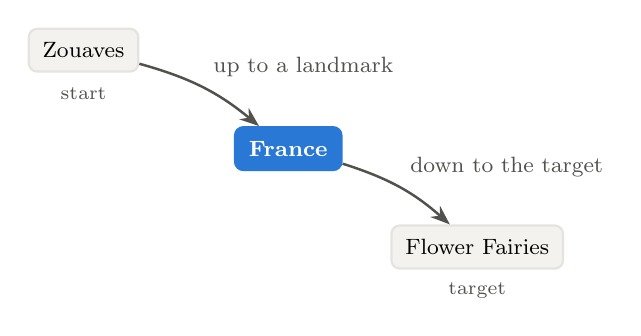
\begin{tikzpicture}[every node/.style={font=\footnotesize},box/.style={draw=rule,line width=0.8pt,rounded corners=3pt,fill=panel,inner sep=5pt}]
  \node[box] (s) at (0,0) {Zouaves};
  \node[box,fill=accent,text=white,draw=accent] (h) at (2.6,-1.25) {\textbf{France}};
  \node[box] (t) at (5.0,-2.5) {Flower Fairies};
  \draw[-{Stealth},ink2,line width=0.9pt] (s) to[bend left=12] node[above right,ink2]{up to a landmark} (h);
  \draw[-{Stealth},ink2,line width=0.9pt] (h) to[bend left=12] node[above right,ink2]{down to the target} (t);
  \node[ink2,font=\scriptsize] at (0,-0.55) {start};
  \node[ink2,font=\scriptsize] at (5.0,-3.05) {target};
\end{tikzpicture}
\end{columns}
\takeaway{\textbf{Question.} Are these intuitive landmarks actually the best hubs for connecting
\emph{any} two articles? If not, which pages are?}
\end{frame}

% ---------- 3. operationalisation ------------------------------------------------------
\begin{frame}{Turning an intuition into two measurable criteria}
\begin{columns}[T,onlytextwidth]
\column{0.47\textwidth}
\kicker{Perceived landmark}
\begin{itemize}
  \item \textbf{out-degree}: distinct articles the page links to
  \item a \textbf{type label}: country, city, list, \dots
\end{itemize}
\vspace{0.3cm}
\kicker{Real hub quality, over random pairs}
\begin{itemize}
  \item \textbf{mean detour} $= d(s,h)+d(h,t)-d(s,t)$\\ \muted{extra clicks paid for going through $h$}
  \item \textbf{on-shortest-path rate}\\ \muted{share of pairs with a detour of 0}
\end{itemize}
\column{0.49\textwidth}
\centering
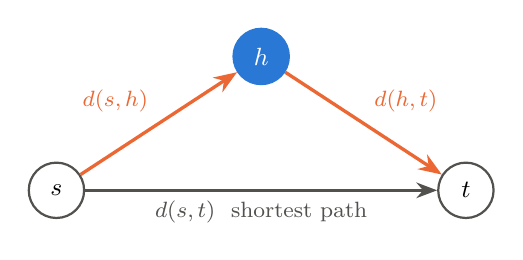
\begin{tikzpicture}[n/.style={circle,draw=ink2,line width=0.8pt,minimum size=20pt,inner sep=0pt,font=\small}]
  \node[n] (s) at (0,0) {$s$};
  \node[n] (t) at (5.2,0) {$t$};
  \node[n,fill=accent,draw=accent,text=white] (h) at (2.6,1.7) {$h$};
  \draw[-{Stealth},line width=1pt,ink2] (s) -- node[below,font=\footnotesize]{$d(s,t)$ \ shortest path} (t);
  \draw[-{Stealth},line width=1.2pt,warm] (s) -- node[above left,font=\footnotesize,warm]{$d(s,h)$} (h);
  \draw[-{Stealth},line width=1.2pt,warm] (h) -- node[above right,font=\footnotesize,warm]{$d(h,t)$} (t);
\end{tikzpicture}

\vspace{0.3cm}
{\footnotesize\muted{Detour $= 0$ means $h$ lies on \emph{at least one} shortest path:\\tied shortest paths need no arbitrary rule.}}
\end{columns}
\takeaway{Only BFS, descriptive statistics and rank comparisons. No machine learning.}
\end{frame}

% ---------- 4. data -------------------------------------------------------------------
\begin{frame}{Data: the complete French Wikipedia link graph}
\begin{columns}[T,onlytextwidth]
\column{0.24\textwidth}\hero{\RawGB\,GB}{5 official dump tables,\\SHA-1 verified}
\column{0.24\textwidth}\hero{14.1\,M}{pages in the dump\\(\NPagesTotal)}\column{0.24\textwidth}\hero{470\,M}{link rows\\(\NLinkRows)}
\column{0.24\textwidth}\hero{\BiasNPages}{pages re-fetched by API\\for a bias check}
\end{columns}
\vspace{0.55cm}
\centering
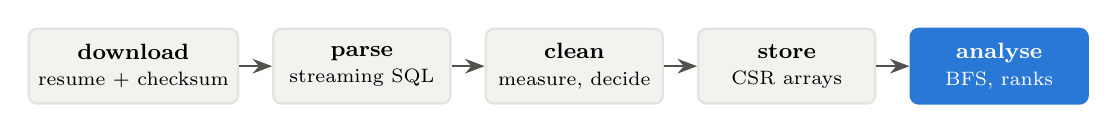
\begin{tikzpicture}[st/.style={rounded corners=3pt,fill=panel,draw=rule,line width=0.8pt,minimum height=0.95cm,minimum width=2.25cm,align=center,font=\footnotesize},
                    node distance=0.42cm]
  \node[st] (a) {\textbf{download}\\\scriptsize resume + checksum};
  \node[st,right=of a] (b) {\textbf{parse}\\\scriptsize streaming SQL};
  \node[st,right=of b] (c) {\textbf{clean}\\\scriptsize measure, decide};
  \node[st,right=of c] (d) {\textbf{store}\\\scriptsize CSR arrays};
  \node[st,right=of d,fill=accent,draw=accent,text=white] (e) {\textbf{analyse}\\\scriptsize BFS, ranks};
  \foreach \x/\y in {a/b,b/c,c/d,d/e} \draw[-{Stealth},ink2,line width=0.9pt] (\x)--(\y);
\end{tikzpicture}
\raggedright
\vspace{0.45cm}
\begin{itemize}
  \item \textbf{Why dumps?} One consistent snapshot (\DumpDate) of \emph{every} link. Crawling would take weeks and mix dates.
  \item \textbf{Why the full graph?} Distances are a global property: sampling the graph would change them. We sample \emph{pairs}.
  \item \textbf{Why French?} It is the edition we play in, and it fits on a laptop.
\end{itemize}
\end{frame}

% ---------- 5. collection pitfall --------------------------------------------------------
\begin{frame}[fragile]{Collection: never assume a schema}
\begin{columns}[T,onlytextwidth]
\column{0.5\textwidth}
\kicker{What we expected (older dumps)}
{\scriptsize
\begin{verbatim}
INSERT INTO `page` VALUES (3,0,'A',..),(7,0,'B',..);
\end{verbatim}
}
\vspace{0.15cm}
\kicker{What the 2026 dump contains}
{\scriptsize
\begin{verbatim}
INSERT INTO `page` VALUES
(3,0,'Antoine_Meillet',0,0,...),
(7,0,'Algèbre_linéaire',0,0,...);
\end{verbatim}
}
\muted{\footnotesize The first parser found \textbf{0 rows}. It failed loudly, so we saw it at once.}
\column{0.45\textwidth}
\kicker{How the parser is made safe}
\begin{itemize}
  \item reads column names from each file's own \texttt{CREATE TABLE}
  \item one strict pattern per row: any surprise raises an error
  \item unit tests on quotes, escapes, UTF-8, NULL
\end{itemize}
\vspace{0.3cm}
\kicker{Independent check}
\hero{0}{rows of difference with a separate\\\texttt{zcat | grep} count, on all 5 tables}
\end{columns}
\end{frame}

% ---------- 6. cleaning -----------------------------------------------------------------
\begin{frame}{Cleaning: measure first, then decide}
\begin{columns}[T,onlytextwidth]
\column{0.61\textwidth}
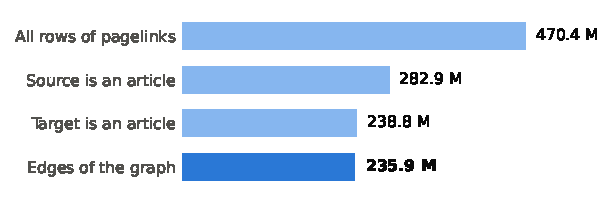
\includegraphics[width=\linewidth]{s_funnel.pdf}\\[0.1cm]
{\footnotesize\muted{Where do the links of articles point?}}\\
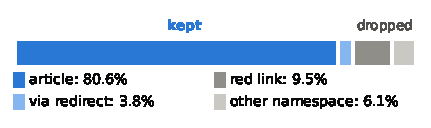
\includegraphics[width=\linewidth]{s_targets.pdf}
\column{0.36\textwidth}
\kicker{One decision per measured problem}
\begin{itemize}\small
  \item \textbf{\NRedirects} redirects among \NNsZeroPages{} main-namespace pages\\ \muted{resolved, longest chain: 3}
  \item \textbf{\ShareRedLinks} red links, \textbf{\ShareLinksOtherNs} other namespaces\\ \muted{impossible moves: dropped}
  \item \textbf{\ShareDuplicates} duplicates after resolution\\ \muted{dropped}
  \item \textbf{\NDisambig} disambiguation pages\\ \muted{traversable, never start/target}
\end{itemize}
\end{columns}
\takeaway{Result: \textbf{\NArticles{} articles} and \textbf{\NEdges{} links}. Sinks (\NSinks) and orphans (\NOrphans) are kept and reported.}
\end{frame}

% ---------- 7. storage -------------------------------------------------------------------
\begin{frame}{Storage: benchmarked on our own queries}
\begin{columns}[T,onlytextwidth]
\column{0.6\textwidth}
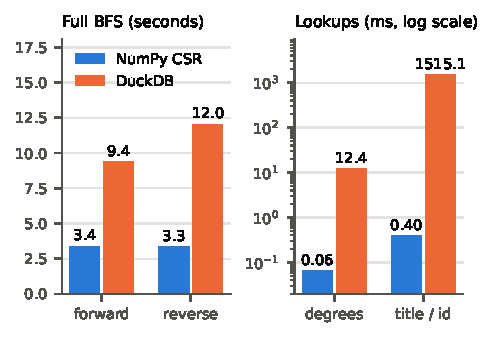
\includegraphics[width=\linewidth]{s_storage.pdf}
\column{0.37\textwidth}
\kicker{Our workload}
A static graph, read only: full BFS runs, degree and title lookups.

\vspace{0.25cm}
\kicker{Observation}
\begin{itemize}\small
  \item CSR: BFS \textbf{\DuckBfsRatio$\times$} to \textbf{\DuckRevBfsRatio$\times$} faster
  \item DuckDB: smaller on disk (\DuckDiskGB{} vs \CsrDiskGB\,GB), opens instantly
\end{itemize}
\vspace{0.25cm}
\kicker{Choice}
\textbf{NumPy CSR + Parquet.}\\
{\small\muted{DuckDB stays for the cleaning joins. Neo4j: a server, and no gain for full BFS.}}
\end{columns}
\end{frame}

% ---------- 8. method --------------------------------------------------------------------
\begin{frame}{Method: random pairs, candidate hubs, exact distances}
\begin{columns}[T,onlytextwidth]
\column{0.58\textwidth}
\kicker{1. Random pairs}
\textbf{\NPairs} pairs $(s,t)$, uniform among articles, fixed seed.\\
\muted{\small Pairs with no path are counted, never dropped.}

\vspace{0.3cm}
\kicker{2. Candidate hubs: \NCandidates{} pages}
\begin{itemize}\small
  \item top \TopK{} by out-degree \muted{(perceived)}
  \item top \TopK{} by in-degree
  \item top \TopK{} by frequency on sampled shortest paths
  \item \NRandomBaseline{} random articles \muted{(baseline)}
\end{itemize}

\vspace{0.2cm}
\kicker{3. Two BFS per hub}
$d(h,\cdot)$ and $d(\cdot,h)$ for all articles give its detour on each pair.
\column{0.38\textwidth}
\centering
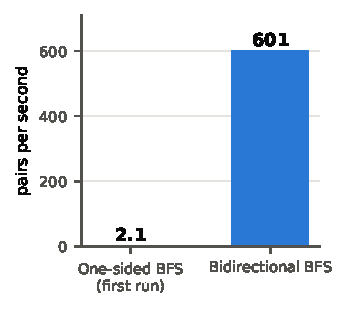
\includegraphics[width=\linewidth]{s_speed.pdf}\\[0.1cm]
{\footnotesize\muted{Searching from both ends at once gives the same exact distances,
\textbf{\PairSpeedup$\times$} faster. The sample grew from \PairsOldN{} to \NPairs{} pairs.}}
\end{columns}
\end{frame}

% ---------- 9. small world ----------------------------------------------------------------
\begin{frame}{First observation: almost everything is four clicks away}
\begin{columns}[T,onlytextwidth]
\column{0.56\textwidth}
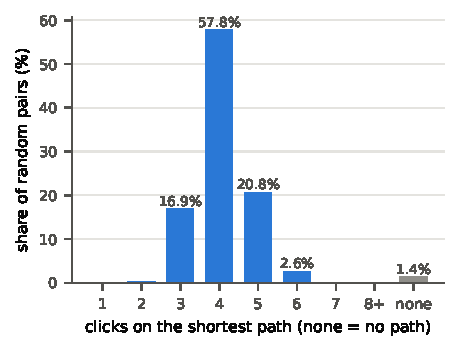
\includegraphics[width=\linewidth]{s_distance.pdf}
\column{0.4\textwidth}
\vspace{0.2cm}
\hero{\MeanDist}{clicks on average between two random articles}

\vspace{0.4cm}
\hero{\LsccShare}{of articles are in one strongly connected component}

\vspace{0.4cm}
\herow{\ShareUnreachable}{of pairs have no path:\\the target is almost always an orphan}
\end{columns}
\end{frame}

% ---------- 10. best hubs -----------------------------------------------------------------
\begin{frame}{Result 1: the best hubs are countries}
\begin{columns}[T,onlytextwidth]
\column{0.7\textwidth}
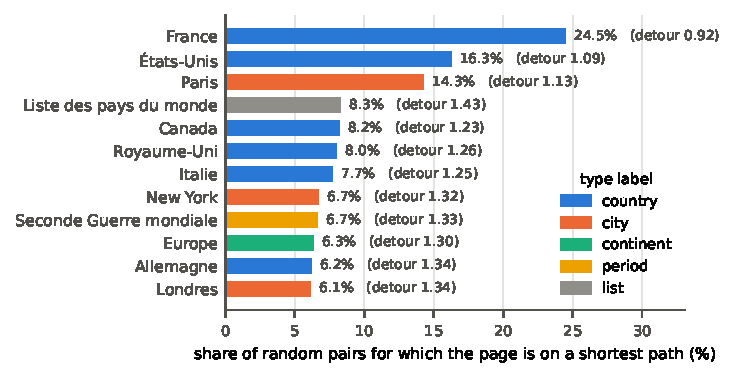
\includegraphics[width=\linewidth]{s_best_hubs.pdf}
\column{0.27\textwidth}
\vspace{0.3cm}
\hero{\BestHubOnPath}{of random pairs have \textbf{\BestHub} on a shortest path}

\vspace{0.45cm}
\hero{\BestHubDetour}{click of detour on average when forced through \BestHub}

\vspace{0.45cm}
{\footnotesize\muted{Best 15 by detour:\\\TopFifteenTypes.}}
\end{columns}
\end{frame}

% ---------- 11. link-rich is not hub -------------------------------------------------------
\begin{frame}{Result 2: many links out does not make a hub}
\begin{columns}[T,onlytextwidth]
\column{0.68\textwidth}
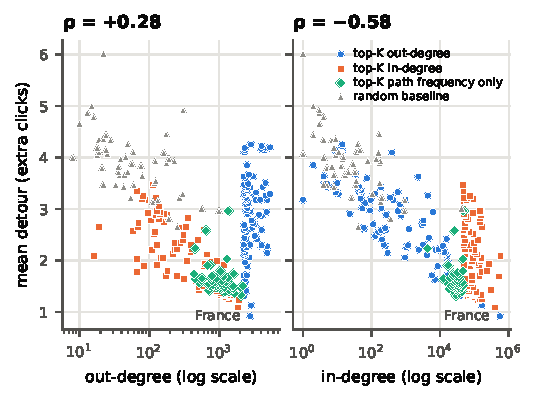
\includegraphics[width=\linewidth]{s_two_scatters.pdf}
\column{0.29\textwidth}
\vspace{0.1cm}
\kicker{Out-degree}
{\small The richest pages are \textbf{lists}: among them, more links mean a \emph{larger} detour. In the other lists, links help.}

\vspace{0.3cm}
\kicker{In-degree}
{\small Being linked \emph{from} many pages tracks hub quality much better.}

\vspace{0.3cm}
\herow{\TopOverlapOutDetour\,/\,\TopOverlapK}{pages shared by the top \TopOverlapK{} by out-degree and the top \TopOverlapK{} by detour}
\end{columns}
\end{frame}

% ---------- 12. types -----------------------------------------------------------------------
\begin{frame}{Result 3: which kinds of pages are good hubs?}
\begin{columns}[T,onlytextwidth]
\column{0.68\textwidth}
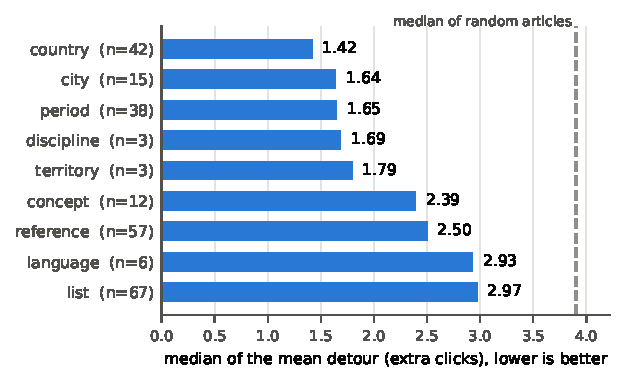
\includegraphics[width=\linewidth]{s_types.pdf}
\column{0.29\textwidth}
\vspace{0.1cm}
\kicker{Observation}
\begin{itemize}\small
  \item countries first
  \item cities and periods next
  \item \emph{reference} pages (ISBN, taxonomic ranks, units): huge in-degree, mediocre hubs
  \item lists last among the large types
\end{itemize}
\vspace{0.2cm}
{\footnotesize\muted{Types cover the \RhoOutDetourN{} non-random candidates. Labels assigned by hand from the page titles. Types with fewer than \MinTypeSize{} pages are merged and not ranked.}}
\end{columns}
\end{frame}

% ---------- 13. bias check --------------------------------------------------------------------
\begin{frame}{Bias check: do templates distort the out-degree?}
\begin{columns}[T,onlytextwidth]
\column{0.5\textwidth}
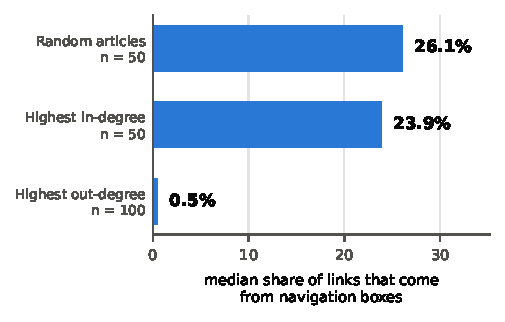
\includegraphics[width=\linewidth]{s_bias_bars.pdf}\\[-2pt]
{\scriptsize\muted{Highest in-degree: countries, reference pages. Highest out-degree: mostly lists.}}
\column{0.47\textwidth}
\kicker{Method}
{\small \BiasNPages{} pages, rendered HTML of the \textbf{exact dump revision} (MediaWiki API). Links counted with and without navigation boxes.}

\vspace{0.3cm}
\kicker{Observations}
\begin{itemize}\small
  \item HTML link count = dump out-degree: median ratio \textbf{\BiasRatioMed} (range \BiasRatioMin--\BiasRatioMax). The measure is validated.
  \item Removing navigation boxes barely changes who is on top ($\rho = \BiasRho$).
\end{itemize}
\end{columns}
\takeaway{Templates do not explain why lists dominate out-degree. We keep template links: they are legal moves.}
\end{frame}

% ---------- 14. robustness ----------------------------------------------------------------------
\begin{frame}{How stable is the ranking?}
\begin{columns}[T,onlytextwidth]
\column{0.4\textwidth}
\centering
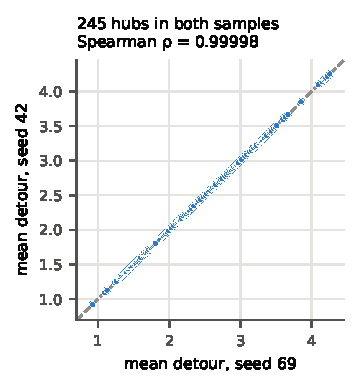
\includegraphics[width=\linewidth]{s_robustness.pdf}
\column{0.56\textwidth}
\vspace{0.2cm}
\kicker{An independent sample gives the same ranking}
\begin{itemize}\small
  \item a second sample of \NPairs{} pairs, drawn with another seed (\OtherSeed), no pair in common
  \item \SeedN{} candidates were evaluated in both: rank correlation \textbf{\SeedRho}
  \item largest change in mean detour: \SeedMaxDiff{} click
  \item the 15 best hubs are the same, \SeedTopFifteenOrder; \OtherBestHub{} is first in both
\end{itemize}

\vspace{0.3cm}
\kicker{Sample size}
{\small\muted{With the first \PairsOldN{} pairs only, the ranking was close
(rank correlation \RobustRho{} with the full sample).}}

\end{columns}
\end{frame}

% ---------- 15. answer ------------------------------------------------------------------------
\begin{frame}{Answer}
\begin{columns}[T,onlytextwidth]
\column{0.47\textwidth}
{\setlength{\fboxsep}{8pt}\colorbox{panel}{\parbox{\dimexpr\linewidth-16pt}{
\kicker{Intuition is right about\dots}
\textbf{the kind of page.}\\[3pt]
{\small Countries, capitals, continents and world wars are the best hubs we found. \BestHub{} leads on both metrics.}}}}
\column{0.47\textwidth}
{\setlength{\fboxsep}{8pt}\colorbox{panel}{\parbox{\dimexpr\linewidth-16pt}{
{\footnotesize\bfseries\color{warm}INTUITION IS WRONG ABOUT\dots}\\[2pt]
\textbf{``pages with many links''.}\\[3pt]
{\small Out-degree mostly measures how much a page \emph{enumerates}. A long list reaches everything in its subject, and little outside it.}}}}
\end{columns}
\vspace{0.45cm}
\kicker{Our interpretation}
\begin{itemize}
  \item A good hub is a page that many articles link \textbf{to}, and that links to broad sub-topics.
  \item Countries have both properties. Lists have only the second, and only inside their subject.
  \item In-degree is a better proxy than out-degree, but not a sufficient one: template-driven reference pages have a huge in-degree and are mediocre hubs.
\end{itemize}\end{frame}

% ---------- 16. limitations & lessons --------------------------------------------------------------
\begin{frame}{Limitations and lessons learned}
\begin{columns}[T,onlytextwidth]
\column{0.48\textwidth}
\kicker{Limitations}
\begin{itemize}\small
  \item hubs evaluated among \NCandidates{} candidates only
  \item type labels are a judgement on page titles
  \item unweighted graph: ignores where a link sits on the page
  \item template links kept as legal moves
  \item structural optimum only: no logs of real games
  \item descriptive statistics, no causal claim
\end{itemize}
\column{0.48\textwidth}
\kicker{Lessons learned}
\begin{itemize}\small
  \item \textbf{Never assume a schema.} The dump layout changed; the parser reads each file's own \texttt{CREATE TABLE}.
  \item \textbf{Measure before cleaning.} Redirect chains were trivial; red links mattered far more.
  \item \textbf{Check the code against its definitions.} Two definitions were wrong at first: the pair populations of the hub metrics, and the unit of the bias check.
  \item \textbf{Pick the algorithm before the hardware.} Bidirectional BFS: \PairSpeedup$\times$.
  \item \textbf{Simple tools fit the scale.} \CsrDiskGB\,GB of arrays, no server.
\end{itemize}
\end{columns}
\end{frame}

% ---------- 17. end ----------------------------------------------------------------------------------
{\setbeamercolor{background canvas}{bg=night}\setbeamertemplate{footline}{}
\begin{frame}[plain]
\centering
{\color{white}\fontsize{24}{28}\selectfont\bfseries Thank you\par}
\vspace{0.4cm}
{\color{white!70!night}\large Questions?\par}
\vspace{1.0cm}
{\color{white!60!night}\footnotesize\texttt{uv run python run.py all} \ reproduces every number and figure of this talk\par}
\end{frame}}

% ---------- backup ------------------------------------------------------------------------------------
\appendix
\begin{frame}{Backup: what would it cost to evaluate every pair?}
\begin{columns}[T,onlytextwidth]
\column{0.31\textwidth}\hero{\AllPairsTrillions\,$\times 10^{12}$}{ordered pairs among \NEligible{} eligible articles}
\column{0.31\textwidth}\herow{\AllPairsYearsBidir{} years}{pair by pair, at \PairRateNew{} pairs per second}
\column{0.31\textwidth}\hero{$\approx$\,\AllPairsDaysBfs{} days}{with one full BFS per start article (\FullBfsWallS\,s each, 6 processes)}
\end{columns}
\vspace{0.6cm}
\begin{itemize}
  \item Extrapolated from the speeds measured on our laptop; not run.
  \item Storing every distance would take about \AllPairsTB\,TB at one byte each, so results would have to be aggregated on the fly.
  \item The ranking was stable from \PairsOldN{} to \NPairs{} pairs: the full computation is not needed for our question.
\end{itemize}
\end{frame}

\begin{frame}{Backup: degrees and a curious cluster}
\begin{columns}[T,onlytextwidth]
\column{0.5\textwidth}
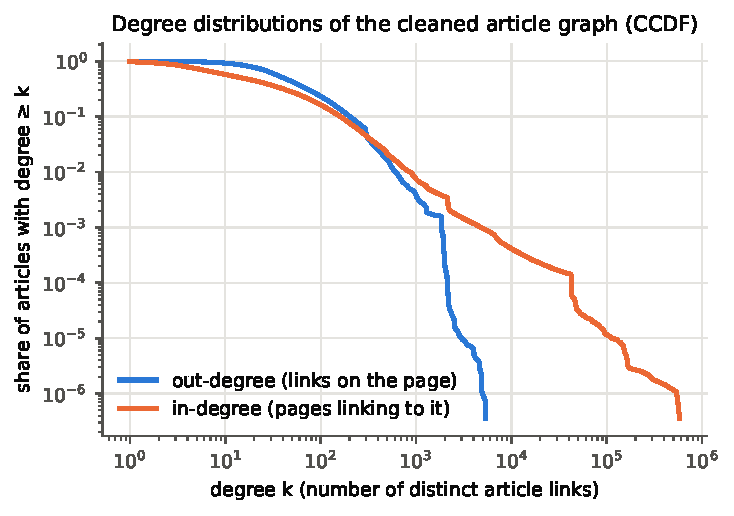
\includegraphics[width=\linewidth]{fig_degree_ccdf.pdf}
\column{0.46\textwidth}
\kicker{Degrees}
\begin{itemize}\small
  \item median out-degree \MedianOutDeg, median in-degree \MedianInDeg
  \item maximum in-degree \MaxInDeg: the authority-control page, linked by a template
\end{itemize}
\vspace{0.3cm}
\kicker{Sexagenary calendar pages}
\begin{itemize}\small
  \item \NSexagenary{} candidates (``Buffle de bois'', \dots)
  \item median out-degree \SexagenaryMedOutDeg, median in-degree \SexagenaryMedInDeg
  \item median detour \SexagenaryMedDetour: many links out, poor hubs
\end{itemize}
\end{columns}
\end{frame}

\begin{frame}{Backup: hub quality by type, all candidates}
\centering
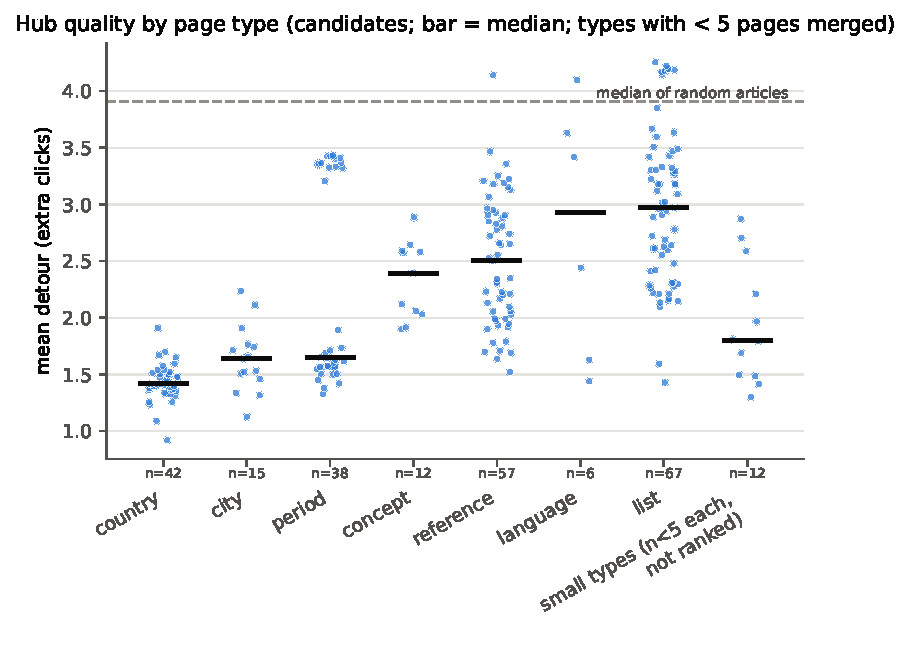
\includegraphics[height=0.74\textheight]{fig_detour_by_type.pdf}
\end{frame}
\end{document}
